\documentclass[11pt]{article} % rozmiar czcionki 11, druk A4
\usepackage{geometry}
\usepackage[utf8]{inputenc}
\usepackage{graphicx}
\usepackage[english, polish]{babel}
\usepackage[T1]{fontenc}
\usepackage{fontspec}
\usepackage[pagestyles]{titlesec}
\usepackage{csquotes}
\usepackage[style=authoryear-ibid,backend=biber]{biblatex}
\setmainfont{Verdana} % czcionka Verdana
\linespread{1.15} % interlinia 1.15
\graphicspath{ {images} }

\addbibresource{sample.bib}

\geometry{twoside, inner=30mm,outer=20mm, top=25mm, bottom=25mm} % marginesy, druk dwustronny
\newpagestyle{mystyle}{\setfoot[\thepage][][]{}{}{\thepage}} %numeracja stron
\pagestyle{mystyle}
\setlength{\parindent}{5mm} % akapit - wcięcie 0.5 cm

\title{Praca inzynierska}
\author{Stanisław Skrzypek}
\date{January 2022}

\begin{document}

\maketitle

\begin{abstract}
    \addcontentsline{toc}{section}{Streszczenie}
    Brak odpowiedniego zarządzania energią w budynkach biurowych od wielu lat 
    powodował straty zarówno finansowe, jak i środowiskowe. Dodatkowo, w wyniku 
    nieodpowiednich warunków panujących w pomieszczeniach pracy, osoby w nich 
    przebywające nie mogły pracować w efektywny sposób. Celem tej pracy było 
    zaproponowanie rozwiązania, za pomocą którego można byłoby mierzyć wartości 
    kluczowych parametrów pomieszczeń biurowych, po czym podejmować stosowne 
    działania mające na celu zarówno poprawienie komfortu pracowników, jak i 
    redukcję zużywanej energii. Wykonano przegląd już istniejących prac naukowych 
    dotyczących optymalnej wartości temperatury oraz natężenia światła w 
    pomieszczeniach biurowych. Przygotowano system informatyczny oparty na 
    architekturze mikrousługowej, który przyjmuje aktualne pomiary i je przetwarza. 
    Przygotowano zestaw czujników, które wykonują pomiary oraz przesyłają 
    je do systemu. 
\end{abstract}

\begin{otherlanguage}{english}
\begin{abstract}
    \addcontentsline{toc}{section}{Summary}
    Lack of proper Energy management in office buildings has caused both 
    financial, as well as environmental loss in many a year. Furthermore, as 
    a result of inadequate room conditions, people staying in those rooms could 
    not work effectively. The aim of this paper was to propose a solution by which 
    it would be possible to measure the values of key parameters of office 
    premises, and then take appropriate actions aimed at both improving the comfort 
    of employees and reducing energy consumption. A review of the already existing 
    scientific works on the optimal value of temperature and light intensity in 
    offices was carried out. An IT system based on a microservice architecture was 
    prepared, which takes current measurements and processes them. A set of sensors 
    has been prepared that perform the measurements and send them to the system.
\end{abstract}
\end{otherlanguage}

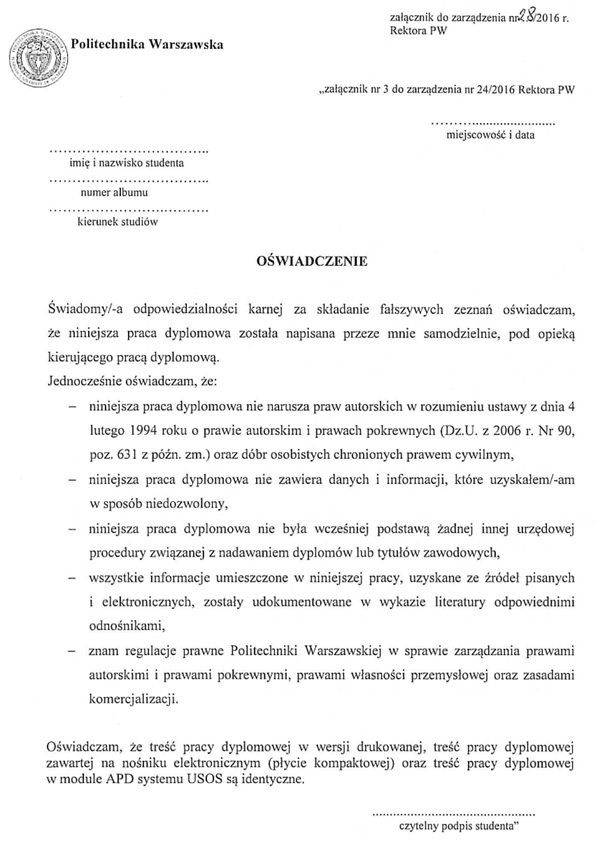
\includegraphics[width=1\textwidth]{oswiadczenie_o_samedzielnosci.jpg}

\tableofcontents

\section{Temat pracy}

Tematem niniejszej pracy jest utworzona w ramach seminarium dyplomowego aplikacja do 
zarządzania warunkami technicznymi w pomieszczeniach biurowych oparta na architekturze 
mikrousługowej. Produkt ma na celu poprawę warunków panujących w pomieszczeniach 
przeznaczonych do pracy codziennej. Wybrane parametry przeznaczone do optymalizacji to 
temperatura oraz natężenie światła.

Implementacja projektu przewiduje umieszczenie w badanych pomieszczeniach odpowiedniego 
rodzaju czujników, które będą na bieżąco monitorować stan danej przestrzeni. 
Zintegrowany z czujnikami system informacyjny powinien odczytywać przesyłane 
pomiary, a następnie je interpretować. Wynik interpretacji powinien być widoczny dla 
zainteresowanych osób. W wiadomości będą znajdować się informacje dotyczące 
akcji, które należy podjąć, aby umożliwić ustalenie się badanych parametrów na 
właściwym poziomie.

Utworzenie aplikacji miało przyczynić się do osiągnięcia dwóch głównych 
celów, stawianych od początku przygotowywania pracy:

\begin{enumerate} % lista numerowana
    \item Poprawa warunków pracy - badania (Oseland i Burton, 2012) dowodzą, że 
    warunki panujące w pomieszczeniach do pracy mają wpływ na efektywność pracowników. 
    Utrzymanie ich na optymalnym poziomie może spowodować wzrost wydajności do 2,5\%
    \item Redukcja zużywanej energii - w praktyce często zdarza się, że po zakończeniu 
    pracy zostawiane są włączone światła na całą noc. Innym przykładem może być 
    sytuacja, w której pomieszczenie jest ogrzewane, mimo iż nikt z niego nie korzysta. 
    Przy wsparciu aplikacji będzie możliwe zapobieganie takim wydarzeniom, co w 
    konsekwencji ograniczy zużycie energii
\end{enumerate}

Zgodnie z wynikami badań opublikowanymi przez Institute for market transformation z 
2016 roku około 40\% całkowitej konsumpcji energii przypada na zasilanie budynków 
(transformation, 2016). Przekłada się to w ciągu roku na wydatek rzędu 450 miliardów 
dolarów. Najsłabiej zagospodarowane budowle zużywały od trzech do siedmiu razy więcej 
energii od tych najbardziej oszczędnych. Istnieje zatem potrzeba przygotowania 
i wdrożenia rozwiązań, które z jednej strony nie byłyby obciążające finansowo, z 
drugiej strony zaś ograniczające już istniejące koszty. 

\section{Istniejące rozwiązania}
Firma Sharp przygotowała podobne rozwiązanie, za pomocą którego można mierzyć kluczowe 
parametry danego pomieszczenia, przesyłać je na platformy chmurowe i je analizować 
(Sharp, 2022). Różnica między tym produktem a rozwiązaniem proponowanym w tej pracy 
polega na tym, że w rozwiązaniu firmy Sharp czujniki są wbudowane w monitor służący 
jako centrum telekonferencyjne. W ten sposób wykonywane pomiary stają się niejako 
dodatkiem do monitora, niż głównym celem wstawienia urządzenia do konkretnej sali. 
W konsekwencji, wykonywanie pomiarów w wielu salach wiązałoby się z koniecznością 
zakupu drogiego monitora dla każdej z nich. Proponowane w tej pracy rozwiązanie zawiera 
jedynie zestaw czujników przesyłających pomiary do systemu, bez innych dodatków, co 
znacznie minimalizuje koszt wdrożenia takiego rozwiązania.
\section{Założenia}
Funkcjonalność i architektura systemu została utworzona w oparciu o kilka istotnych 
założeń:

\begin{itemize} % lista nienumerowana
    \item Łatwość wdrożenia - system powinien być gotowy do wdrożenia na środowisko 
    chmurowe. Organizacja zainteresowana uruchomieniem aplikacji dla swoich potrzeb 
    może wybrać opcję, w której dostarczane są obrazy odpowiednich serwisów oraz 
    skrypty konfigurujące środowisko. Takie rozwiązanie mogłoby być ofertą skierowaną 
    do banków, które chcą zminimalizować ruch zewnętrzny. Może także skorzystać z 
    opcji, w której system jest hostowany na serwerach firmy będącej autorem 
    oprogramowania
    \item System składa się z czujników zbierających pomiary, które następnie przesyłane 
    są do serwisów, które je przetwarzają. Do pomiaru zalicza się aktualna 
    temperatura, natężenie światła oraz jakość powietrza
    \item Aplikacja oparta jest na regułach określających oczekiwaną wartość powyższych 
    parametrów w danej chwili czasu. Po otrzymaniu każdego z pomiarów porównywane są 
    wartości oczekiwane z rzeczywistymi i na tej podstawie aplikacja przygotowuje wynik. 
    Domyślnie istnieje reguła podstawowa, gdzie oczekiwana temperatura wynosi 24,50. 
    Więcej informacji odnośnie tego skąd taka wartość została ustalona można 
    uzyskać, patrząc na tabelę 1
    \item System przewiduje dwie role użytkowników: pracowników danej 
    organizacji, którzy mogą tworzyć własne reguły dla pomieszczeń do nich 
    przypisanych, oraz administratorów organizacji, którzy posiadają wszystkie 
    uprawnienia przypisane pracownikom, a ponadto możliwość zarządzania informacjami 
    dotyczącymi organizacji, budynków, pomieszczeń i czujników
\end{itemize}

\section{Metodologia}
\subsection{Architektura systemu}
\subsubsection{Serwisy zorientowane usługowo}
\subsubsection{Sprzężenie serwisów}
\subsubsection{Architektura systemu do zarządzania energią w pomieszczeniach biurowych}
\section{Przechowywanie danych}
\subsection{MySQL}
\subsubsection{Schemat adresów}
\subsubsection{Schemat organizacji}
\subsubsection{Schemat reguł}
\subsubsection{Schemat sensorów}
\subsubsection{Schemat użytkowników}
\subsection{InfluxDB}
\section{Komunikacja między serwisami}
\subsection{Broker wiadomości}
\subsubsection{MassTransit}
\subsection{Styki}
\subsubsection{Styk mikrousługi danych adresów}
\subsubsection{Styk mikrousługi danych organizacji}
\subsubsection{Styk mikrousługi danych reguł}
\subsubsection{Styk mikrousługi danych sensorów}
\subsubsection{Styk mikrousługi mikrousługi aplikacyjnej administratorów}
\section{Testy}
\subsection{Testy jednostkowe}
\subsection{Testy integracyjne}
\subsection{Testy end-2-end}
qwe

0jakis tekst
000jakis tekst

\subsection{Automatyzacja testów}
jakis tekst
\section{Automatyzacja}
1jakis tekst
\subsection{Automatyzacja wdrożenia}
2jakis tekst
\subsection{Ciągła integracja}
3jakis tekst
\subsection{Ciągłe dostarczanie}
4jakis tekst
\subsection{Kubernetes}
\subsubsection{Komponenty płaszczyzny sterowania}
\subsubsection{Komponenty węzła}
\section{Podsumowanie}
\subsection{Możliwości rozszerzenia projektu}
\section{Bibliografia}
\printbibliography
\section{Wykaz symboli i skrótów}
\section{Spis rysunków}
\section{Spis tabel}
\section{Spis załączników}

\begin{enumerate}
    \item 1A citation command in parentheses: \parencite{Smith:2012qr}.
    \item 2A citation command for use in the flow of text: As \textcite{Smith:2013jd} said \dots
    \item 3A citation command which automatically switches style depending on location and the option setting in the package declaration (see line 12 in the LaTeX source code). In this case, it produces a citation in parentheses: \autocite{Other:2014ab}.
    \end{enumerate}

\end{document}